\documentclass{article}
\textwidth 15cm
\usepackage{graphicx}
\usepackage{hyperref}
\title{Numerical explorations in a modified potential of the TBP}
\author{F. J.~Mu\~noz-Almaraz\footnote{Universidad CEU-Cardenal
    Herrera}, J.~Gal\'an-Vioque\footnote{Universidad de Sevilla},
  E.~Freire\footnotemark[2]%\footnote{Universidad de Sevilla}
  ,
  A.~Vanderbawhede\footnote{University of Gent}}
\begin{document}
\maketitle
\begin{abstract}
  This is a working document distributed in 2005 among our group and other
  researchers interested about bifurcation for numerical continuation
  of modified potential of the three body problem (TBP) starting from
  the figure-8\cite{Ocho}. In 2018, Dr.~Toshiaki Fujiwara told us that he was
  going to cite our private communication about this topic. Therefore,
 this document is making publicly available that communication as well
 as the code for numerical continuation  with AUTO. The body of this
 document consists in the working document of 2005, adding some
 remarks as footnotes and a bibliography with the papers where the
 algoritm are described. 
\end{abstract}
We are going to study central forces 
\begin{equation}
H=\frac 1 2 (\| \mathbf{p}_1\|^2 +\| \mathbf{p}_2\|^2+ \| \mathbf{p}_3\|^2) - \frac 1 {\|  \mathbf{q}_1-\mathbf{q}_2\|^{\alpha}}
-\frac 1 {\|  \mathbf{q}_1-\mathbf{q}_3\|^{\alpha}}-\frac 1 {\|  \mathbf{q}_2-\mathbf{q}_3\|^{\alpha}}
\end{equation}
where $\mathbf{p}_1$, $\mathbf{p}_2$, $\mathbf{p}_3$, $\mathbf{q}_1$, $\mathbf{q}_2$ and  $\mathbf{q}_3$ 
are vectors on the plane.
  
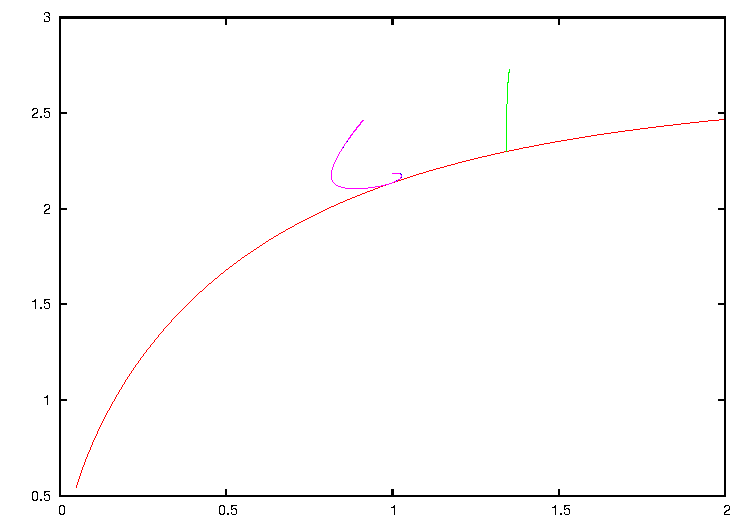
\includegraphics{bd.pdf}

The bifurcation diagram displayed above has as horizontal axis the exponent in the potential of Hamiltonian, $\alpha$, 
and the vertical axis is the norm $L^2$ given by AUTO as output. I do not know why it could not be the pink curve and  the red curve tangent.
The red curve is the family where the figure-eight is. This red family goes from $\alpha=1$ up to very high values for $\alpha$, in the other 
direction is going to go from $\alpha=1$ up to close to $\alpha=0$. Every orbit in the family is the three bodies following a curve with figure eight. 
Characteristic multipliers are shown in the following figure

\begin{tabular}{cc}
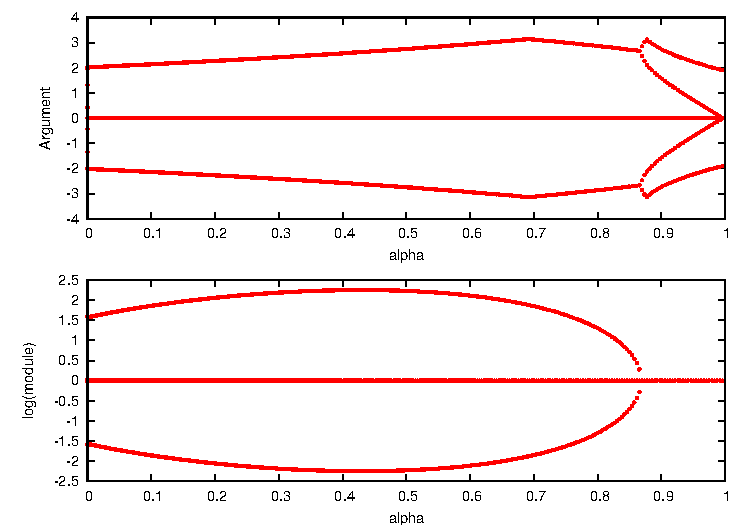
\includegraphics[width=0.45\textwidth]{cm_down.pdf}&
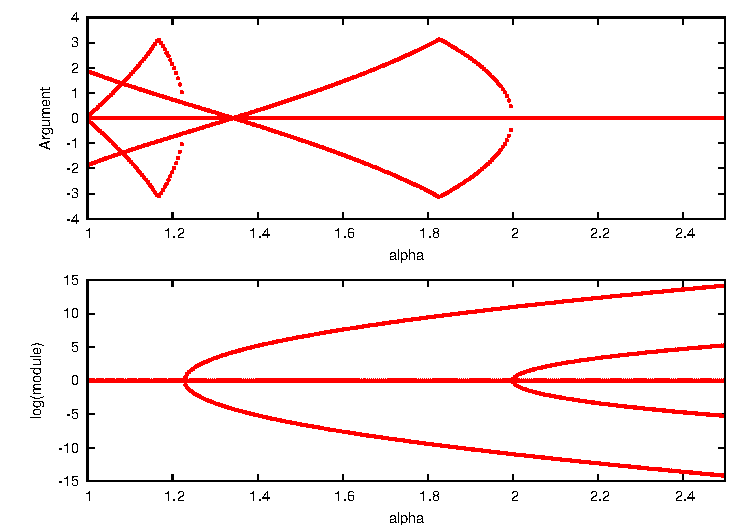
\includegraphics[width=0.45\textwidth]{cm_up.pdf}
\end{tabular}

The red family is symmetric with respect to the two time-reversal
symmetries of the figure eight\footnote{The general procedure and its
  theoretical explanation of
  continuation with time--reversal symmetries is described in
  \cite{CelMech}. These techniques are applied for the TBP in
  \cite{Zaragoza} to calculate numerical continuation starting from
  the eight orbits. The two time--reversal symmetries are described
  there depeding on the matrix we use $S_{M_1}=\left [
    \begin{array}{cc}
      1  & 0 \\
      0 & -1
    \end{array} ] \right ] $ or $S_{E_1}=\left [
    \begin{array}{cc}
      -1  & 0 \\
      0 & -1
    \end{array} ] \right ] $
}. The continuation 
with both of them allows us to find two bifurcation points at $\alpha= 0.996562$  and $\alpha= 1.34242$. However, the other two bifurcation 
are not detected with the symmetric continuation and with the method
for period orbit.
\footnote{Detection of bifurcation with the method of continuation
  explained in~\cite{PhysD} is very sensitive and not always is
  detecting bifurcations.  There are there values where a change of
  stability is undergoing according to the characteristics
  multipliers:
  $\alpha=0.8\dots$, $\alpha=1.2283$ and $\alpha=2$, they are
  undetected with the time-reversal continuation schemes. We have studied
  in \cite{Istambul} a situation with change of stability without
  branching. We have not studied whether or not this is the situation
  for these values.}
The two detected bifurcation have a 
``passing'' behauvior (the characteristic multiplier pass through the one and stays on the unit circle) and the undetected are ``splitting'' (there exists a
change in the linear stability). The undetected are more or less close to $\alpha=1.2283$ and $\alpha=2$. Is $\alpha=2$ a special point?

From the bifurcation point at $\alpha= 0.996562$, a family of doubly symmetric periodic orbits appears. In the diagram is the pink curve. 
This family looks like tangent to the red curve, I should check it. I do not understand which is the reason because of these curves can not be tangent. I would thank an explanation.  Here some orbits of the family in a direction:

\begin{tabular}{cc}
\includegraphics[width=0.45\textwidth]{./orbits/o1.pdf}&
\includegraphics[width=0.45\textwidth]{./orbits/o2.pdf} \\
$\alpha= 0.98974558119$&$ \alpha=0.97657871845 $
\end{tabular}

\begin{tabular}{cc}
\includegraphics[width=0.45\textwidth]{./orbits/o3.pdf}&
\includegraphics[width=0.45\textwidth]{./orbits/o4.pdf}\\
$\alpha= 0.92520305647$&$ \alpha= 0.86299535233$
\end{tabular}

\begin{tabular}{cc}
\includegraphics[width=0.45\textwidth]{./orbits/o5.pdf}&
\includegraphics[width=0.45\textwidth]{./orbits/o6.pdf}\\
$\alpha= 0.81555487427$&$ \alpha=0.84462774170 $
\end{tabular}

\begin{tabular}{cc}
\includegraphics[width=0.45\textwidth]{./orbits/o7.pdf}&
\includegraphics[width=0.45\textwidth]{./orbits/o8.pdf}\\
$\alpha=0.88342919391 $&$ \alpha=0.90984042548 $
\end{tabular}

In the opposite direction from the bifurcation, we have displayed some periodic orbits: 

\begin{tabular}{cc}
\includegraphics[width=0.45\textwidth]{./orbits/b1.pdf}&
\includegraphics[width=0.45\textwidth]{./orbits/b2.pdf}\\
$\alpha=1.0025843346 $&$ \alpha= 1.0101864584$
\end{tabular}

\begin{tabular}{cc}
\includegraphics[width=0.45\textwidth]{./orbits/b3.pdf}&
\includegraphics[width=0.45\textwidth]{./orbits/b4.pdf}\\
$\alpha= 1.0215325651$&$ \alpha= 1.0265396023$
\end{tabular}

\begin{tabular}{cc}
\includegraphics[width=0.45\textwidth]{./orbits/b5.pdf}&
\includegraphics[width=0.45\textwidth]{./orbits/b6.pdf}\\
$\alpha= 1.0265820623$&$ \alpha= 1.0244124526$
\end{tabular}

\begin{tabular}{cc}
\includegraphics[width=0.45\textwidth]{./orbits/b7.pdf}&
\includegraphics[width=0.45\textwidth]{./orbits/b8.pdf}\\
$\alpha= 1.0137412091$&$ \alpha= 1.0005848879$
\end{tabular}

About the above family, I am surprised because they look like the orbits in the family which belongs the figure eight when one of the  masses is varied. 

From the other bifurcation  at $\alpha= 1.34242$ appears the family which correspond to the green curve in the above bifurcation diagram. This family is also symmetric with respect to the two time-reversal symmetries.  Again, there are some orbits from this family.

\begin{tabular}{cc}
\includegraphics[width=0.45\textwidth]{./orbits/orb1.pdf}&
\includegraphics[width=0.45\textwidth]{./orbits/orb2.pdf}\\
$\alpha=1.3424242750 $&$ \alpha=1.3424432064 $
\end{tabular}

\begin{tabular}{cc}
\includegraphics[width=0.45\textwidth]{./orbits/orb3.pdf}&
\includegraphics[width=0.45\textwidth]{./orbits/orb4.pdf}\\
$\alpha= 1.3425063709$&$ \alpha=1.3426429099 $
\end{tabular}

\begin{tabular}{cc}
\includegraphics[width=0.45\textwidth]{./orbits/orb5.pdf}&
\includegraphics[width=0.45\textwidth]{./orbits/orb6.pdf}\\
$\alpha=1.3429612329 $&$ \alpha=1.3439693118 $
\end{tabular}

\begin{tabular}{cc}
\includegraphics[width=0.45\textwidth]{./orbits/orb7.pdf}&
\includegraphics[width=0.45\textwidth]{./orbits/orb8.pdf}\\
$\alpha= 1.3470762333$&$ \alpha= 1.3504602980$
\end{tabular}

\begin{thebibliography}{99}
  \bibitem{Ocho} Chenciner, A. \& Montgomery, R. (2000). \textit{A remarkable periodic solution of the three-body problem in the case of equal masses}. Annals of Mathematics-Second Series, 152(3), 881-902.\url{http://emis.ams.org/journals/Annals/152_3/chencine.pdf}
\bibitem{PhysD} Mu\~{n}oz-Almaraz, F. J., Freire, E., Gal\'an,
  J., Doedel, E., \& Vanderbauwhede, A. (2003). \textit{Continuation of
  periodic orbits in conservative and Hamiltonian systems}. Physica D:
  Nonlinear Phenomena, 181(1–2),
  1–38. \url{https://doi.org/10.1016/S0167-2789(03)00097-6}
\bibitem{Zaragoza}  Mu\~noz–Almaraz, F. J., Gal\'an-Vioque, J., \& Freire, E. (2004). \textit{Families of symmetric periodic orbits in the three body problem and the figure eight}. Monograf\'ias de La Real Academia de Ciencias de Zaragoza, 25, 229–240.
  \bibitem{CelMech} Mu\~noz-Almaraz, F. J., Freire, E., Gal'an-Vioque,
  J., \& Vanderbauwhede, A. (2007). Continuation of normal doubly
  symmetric orbits in conservative reversible systems. Celestial
  Mechanics and Dynamical Astronomy, 97(1),
  17–47. \url{https://doi.org/10.1007/s10569-006-9048-3}
 \bibitem{Istambul} Mu\~noz–Almaraz, F. J., Freire, E., Gal\'an-Vioque, J., \& Vanderbauwhede, A. (2009). \textit{Change of Stability withour Bifurcation: An Example}. In Proceedings of the 14th International Conference on Difference Equations and Applications (pp. 3–18). Istambul. Turkey: Ugur-Bahcesehir University Publishing.
\end{thebibliography}
\end{document} 